\subsubsection{Algorithm Classes}

\begin{figure}[h]
	\centering
	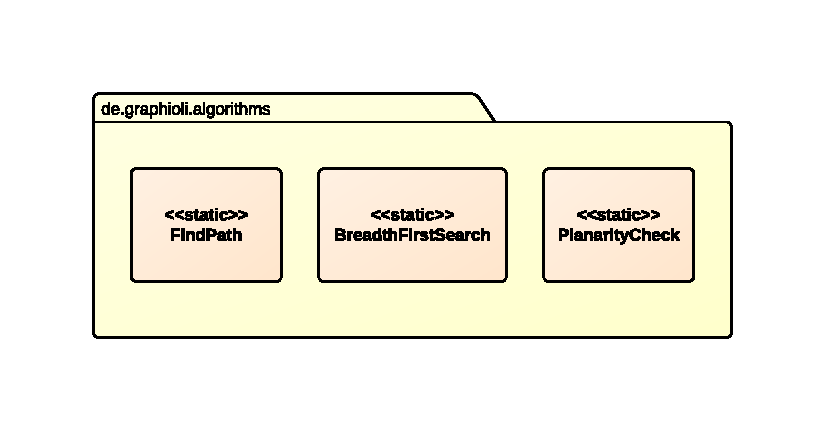
\includegraphics[page=1,width=\textwidth,keepaspectratio]{algorithmsClassDiagram.pdf}
	\caption{Algorithm class diagram.}
	\label{img:algorithmsClassDiagram}
\end{figure}
%\pagebreak

% FindPath
\static{FindPath}{findpath}
This class is part of the \texttt{de.graphioli.algorithms} package and is able to check if there is a path between two given \texttt{vertices}. \\

\centerdash

\paragraph*{Method Summary}
\paragraph*{}
\begin{longtable}{Lp{10cm}}
	\startmethodtable
	\method{public boolean}{performAlgorithm(Graph graph, Vertex vertexA, Vertex vertexB)}{fp:performalgorithm} \\
	& Returns \texttt{true} if there is a path in the specified \ref{cls:graph} between the two specified \texttt{vertices} \texttt{vertexA} and \texttt{vertexB}. \\
	\hline
\end{longtable}

% BreadthFirstSearch
\static{BreadthFirstSearch}{breadthfirstsearch}
This class is part of the \texttt{de.graphioli.algorithms} package and is able to perform the \gls{BFS} algorithm. \\

\centerdash

\paragraph*{Method Summary}
\paragraph*{}
\begin{longtable}{Lp{10cm}}
	\startmethodtable
	\method{public Iterable<Vertex>}{performAlgorithm(Graph graph, Vertex vertex, int depth)}{bfs:performalgorithm} \\
	& Performs the \gls{BFS} algorithm on the specified \ref{cls:graph} with the specified \ref{cls:vertex} and \texttt{depth}, and returns an iterable list of  traversed \texttt{vertices}. \\
	\hline
\end{longtable}

% PlanarityCheck
\static{PlanarityCheck}{planaritycheck}
This class is part of the \texttt{de.graphioli.algorithms} package and is able to check if a drawing of a \ref{cls:graph} is planer. \\

\centerdash

\paragraph*{Method Summary}
\paragraph*{}
\begin{longtable}{Lp{10cm}}
	\startmethodtable
	\method{public boolean}{performAlgorithm(GameBoard board)}{pc:performalgorithm} \\
	& Returns \texttt{true} if the specified \ref{cls:gameboard} is drawn planarly. \\
	\hline
\end{longtable}
